\documentclass[12pt,letterpaper]{report}
\usepackage{natbib}
\usepackage{geometry}
%\usepackage{fancyheadings} fancyheadings is obsolete: replaced by fancyhdr. JL
\usepackage{fancyhdr}
\usepackage{afterpage}
\usepackage{graphicx}
\usepackage{amsmath,amssymb,amsbsy}
\usepackage{dcolumn,array}
\usepackage{tocloft}
\usepackage{asudis}

\begin{document}
%-----------------------front matter
\pagenumbering{roman}
\title{Challenge Task 2018}
\subtitle{Implementation of a Decentralized Application Tic Tac Toe}
\paperType{Dissertation}
\chair{Departements of Informatics - Communication Systems Group}
\memberOne{Lucas Pelloni, leginumeber}
\memberTwo{Severin Wullschleger leginumber}
\memberThree{Andreas Schaufelbühl, 12-918-843}

\maketitle
\doublespace
%\begin{abstract}
\end{abstract}

\dedicationpage{}
%\include{ack}
\tableofcontents
% This puts the word "Page" right justified above everything else.
\addtocontents{toc}{~\hfill Page\par}
% Asking LaTeX for a new page here guarantees that the LOF is on a separate page
% after the TOC ends.
\newpage
% Making the LOT and LOF "parts" rather than chapters gets them indented at
% level -1 according to the chart: top of page 4 of the document at
% ftp://tug.ctan.org/pub/tex-archive/macros/latex/contrib/tocloft/tocloft.pdf
\addcontentsline{toc}{part}{LIST OF TABLES}
\renewcommand{\cftlabel}{Table}
\listoftables
% This gets the headers for the LOT right on the first page.  Subsequent pages
% are handled by the fancyhdr code in the asudis.sty file.
\addtocontents{lot}{Table~\hfill Page \par}
\newpage
\addcontentsline{toc}{part}{LIST OF FIGURES}
\addtocontents{toc}{CHAPTER \par}
\renewcommand{\cftlabel}{Figure}
\listoffigures
% This gets the headers for the LOF right on the first page.  Subsequent pages
% are handled by the fancyhdr code in the asudis.sty file.
\addtocontents{lof}{Figure~\hfill Page \par}
%-----------------------body
\doublespace
\pagenumbering{arabic}
\chapter{Introduction}\label{ch:introduction}
%introduce to the task and idea
This years Challenge Task is to implement a Decentralized Application (DApp) running in the Ethereum blockchain. The goal of the application is a playable Tic-Tac-Toe\footnote{https://en.wikipedia.org/wiki/Tic-tac-toe} game, which also includes a betting system, all embedded in a Smart Contract.
\\\\
%Introduce more our project here

Chapter \ref{ch:technologies} gives an overview and short explanation of the technologies we use in order to implement the Challenge Task.\\
In Chapter \ref{ch:implementation} we show the actual implementation of the game. It starts by explaining and showing our project structure. Also we give walk-through of the different processes of playing a game and betting on games.\\
The problems and challenges occurred within our project are discussed in Chapter \ref{ch:discussion}. Additionally we also describe our open task and goals for the future concerning this project.
\chapter{Technologies}\label{ch:technologies}
With Solidity\footnote{https://github.com/ethereum/solidity} we implement the \ac{sc} which will run on the Ethereum blockchain platform. For our front-end we choose using React\footnote{https://reactjs.org/}, which is a JavaScript library for building user interfaces. The interaction of the front-end application with our \ac{sc} is provided through Web3.js\footnote{https://web3js.readthedocs.io/en/1.0/} and MetaMask\footnote{https://metamask.io/}. To speed up the testing and development we use Ganache\footnote{http://truffleframework.com/ganache/} to run our local Etherum blockchain
In the following section we describe the different technologies and its use in our project more in detail.
\section{Solidity}
\section{Web3.js}
\section{MetaMask}
\section{Ganache}
%which technologies are used and why --> should we go into detail? maybe a chart showing how they interact?

\chapter{Implementation of the game}\label{ch:implementation}
\section{The Smart Contract}
\noindent The class-diagram in Figure\ref{fig:sc_uml}  show a detail class diagram explaining the modelling and structure of our \ac{sc}. \\
\begin{figure}[ht]
	\begin{center}
		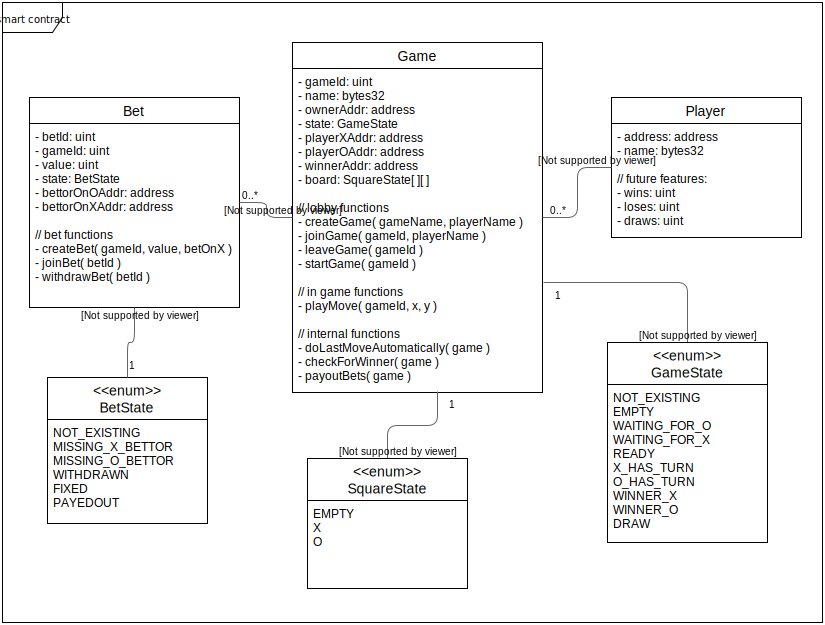
\includegraphics[scale=0.22]{res/sc_uml}
	\end{center}
	\caption{Class-Diagram of the \ac{sc}}
	\label{fig:sc_uml}
\end{figure}\newline
\noindent The \ac{sc} can hold multiple games, which always contain one board and two players. Every time time a user opens up a new Game, he automatically gets assigned as one of the playing party. Now the Game state is automatically set to 'WAITING\_FOR\_X'. As soon as a second player chooses to enter a open game, the game owner can start the game, which changes the state to 'X\_HAS\_TURN' as the game has now started and the guest player has to do his first move.\\\\
All Bets contain a game-id pointing to the game the bet is referencing on it. The user who creates a bet chooses the game and the amount of token he want to bet with and pays it into the \ac{sc}. Is there an opponent bettor joining the bet is changing to the state 'FIXED'.\\
If the game finds an end the state of it changes to either 'WINNER\_X', 'WINNER\_O' or 'DRAW', which activates the function 'payout' ,triggering all bets referencing to this particular game. So the bets will change the state to 'PAYOUT' and user will get paid according to their betting.\\ 
Three functions of the \ac{sc} we show here, to discuss in detail the implementation and structure of the \ac{sc}:\\





%logic and modell

\chapter{Discussion}\label{ch:discussion}
\section{Challenges and Problems}
As the language of solidity is pretty new, the functionalities are quiet limited. Writing the \ac{sc} we were facing the problem of not being able to transact strings from \ac{sc} to the front-end and reverse. Yet we could achieve the same result with sending bytes32 data and transform them in the front-end. So we are able to store strings as game name, player name etcetera.\\
Also the lack of good documentation was sometimes raising up some challenges, although with the help of StackOverFlow\footnote{https://stackoverflow.com/} most of the problems found their solutions.
\section{Future work}
\noindent Our goal is to release our game on the Ethereum main network. A major challenge in order to achieve that is the reduction of the amount of gas required. All the different transaction are not optimized in terms of minimal gas reduction. Also the code in our \ac{sc} is very long. As a result the gas usage of transaction is high.\newline
To tackle this problem Prof. Thomas Bocek will audit our \ac{sc}, so we can achieve with his help and guidance an major gas reduction.\\\\
Besides some minor GUI improvements a second goal is to get an free https certificate with deploying our game through GitHub Pages\footnote{https://pages.github.com/}.
As a third goal we aim to submit  our \ac{dapp} to State of the Apps\footnote{https://www.stateofthedapps.com/}, a platform for open \ac{dapp}'s, so we reach a broader blockchain audience and let them play and bet on our game.

\include{chapter5}
\include{chapter6}
%-----------------------back matter
{\singlespace
% Making the references a "part" rather than a chapter gets it indented at
% level -1 according to the chart: top of page 4 of the document at
% ftp://tug.ctan.org/pub/tex-archive/macros/latex/contrib/tocloft/tocloft.pdf
\addcontentsline{toc}{part}{REFERENCES}
\bibliographystyle{asudis}
\bibliography{dis}}
\renewcommand{\chaptername}{APPENDIX}
\addtocontents{toc}{APPENDIX \par}
\appendix
\chapter{Raw Data}

\include{vita}
\end{document}
